% Created by tikzDevice version 0.12
% !TEX encoding = UTF-8 Unicode
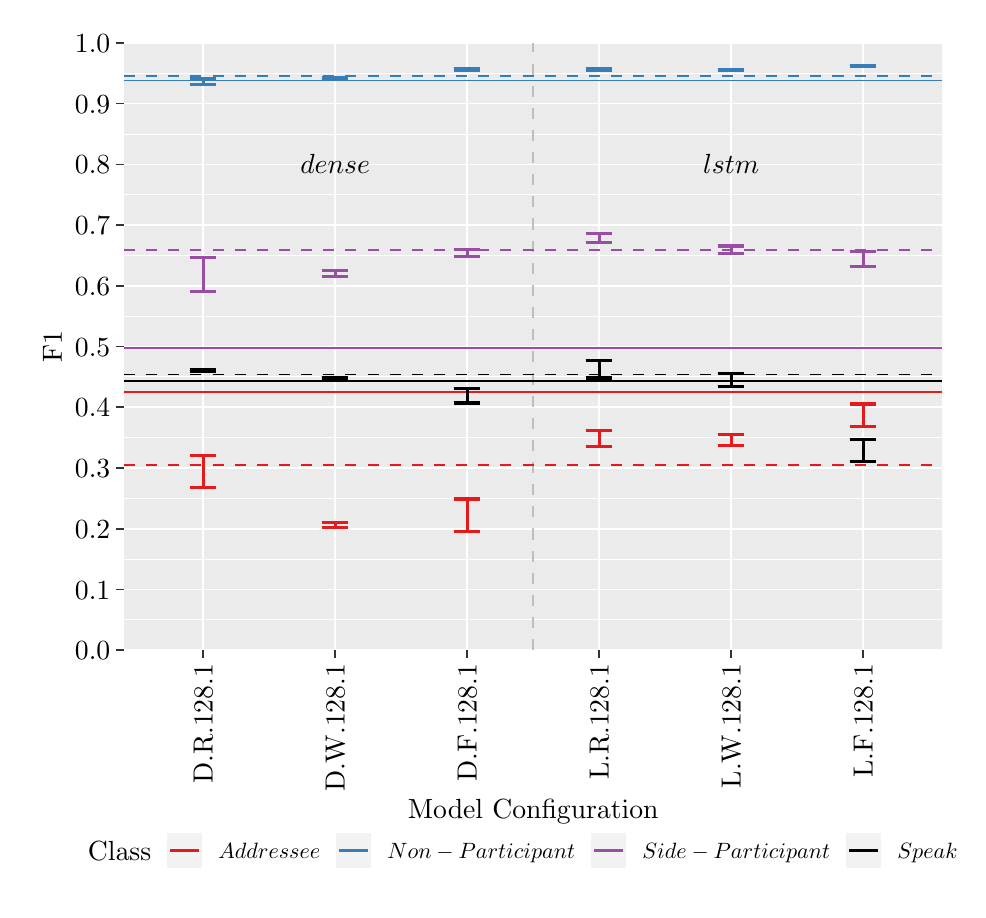
\begin{tikzpicture}[x=1pt,y=1pt]
\definecolor{fillColor}{RGB}{255,255,255}
\path[use as bounding box,fill=fillColor,fill opacity=0.00] (0,0) rectangle (336.00,311.47);
\begin{scope}
\path[clip] (  0.00,  0.00) rectangle (336.00,311.47);
\definecolor{drawColor}{RGB}{255,255,255}
\definecolor{fillColor}{RGB}{255,255,255}

\path[draw=drawColor,line width= 0.6pt,line join=round,line cap=round,fill=fillColor] (  0.00,  0.00) rectangle (336.00,311.47);
\end{scope}
\begin{scope}
\path[clip] ( 34.81, 86.52) rectangle (330.50,305.97);
\definecolor{fillColor}{gray}{0.92}

\path[fill=fillColor] ( 34.81, 86.52) rectangle (330.50,305.97);
\definecolor{drawColor}{RGB}{255,255,255}

\path[draw=drawColor,line width= 0.3pt,line join=round] ( 34.81, 97.49) --
	(330.50, 97.49);

\path[draw=drawColor,line width= 0.3pt,line join=round] ( 34.81,119.44) --
	(330.50,119.44);

\path[draw=drawColor,line width= 0.3pt,line join=round] ( 34.81,141.38) --
	(330.50,141.38);

\path[draw=drawColor,line width= 0.3pt,line join=round] ( 34.81,163.33) --
	(330.50,163.33);

\path[draw=drawColor,line width= 0.3pt,line join=round] ( 34.81,185.27) --
	(330.50,185.27);

\path[draw=drawColor,line width= 0.3pt,line join=round] ( 34.81,207.22) --
	(330.50,207.22);

\path[draw=drawColor,line width= 0.3pt,line join=round] ( 34.81,229.16) --
	(330.50,229.16);

\path[draw=drawColor,line width= 0.3pt,line join=round] ( 34.81,251.11) --
	(330.50,251.11);

\path[draw=drawColor,line width= 0.3pt,line join=round] ( 34.81,273.05) --
	(330.50,273.05);

\path[draw=drawColor,line width= 0.3pt,line join=round] ( 34.81,295.00) --
	(330.50,295.00);

\path[draw=drawColor,line width= 0.6pt,line join=round] ( 34.81, 86.52) --
	(330.50, 86.52);

\path[draw=drawColor,line width= 0.6pt,line join=round] ( 34.81,108.46) --
	(330.50,108.46);

\path[draw=drawColor,line width= 0.6pt,line join=round] ( 34.81,130.41) --
	(330.50,130.41);

\path[draw=drawColor,line width= 0.6pt,line join=round] ( 34.81,152.36) --
	(330.50,152.36);

\path[draw=drawColor,line width= 0.6pt,line join=round] ( 34.81,174.30) --
	(330.50,174.30);

\path[draw=drawColor,line width= 0.6pt,line join=round] ( 34.81,196.25) --
	(330.50,196.25);

\path[draw=drawColor,line width= 0.6pt,line join=round] ( 34.81,218.19) --
	(330.50,218.19);

\path[draw=drawColor,line width= 0.6pt,line join=round] ( 34.81,240.14) --
	(330.50,240.14);

\path[draw=drawColor,line width= 0.6pt,line join=round] ( 34.81,262.08) --
	(330.50,262.08);

\path[draw=drawColor,line width= 0.6pt,line join=round] ( 34.81,284.03) --
	(330.50,284.03);

\path[draw=drawColor,line width= 0.6pt,line join=round] ( 34.81,305.97) --
	(330.50,305.97);

\path[draw=drawColor,line width= 0.6pt,line join=round] ( 63.42, 86.52) --
	( 63.42,305.97);

\path[draw=drawColor,line width= 0.6pt,line join=round] (111.11, 86.52) --
	(111.11,305.97);

\path[draw=drawColor,line width= 0.6pt,line join=round] (158.81, 86.52) --
	(158.81,305.97);

\path[draw=drawColor,line width= 0.6pt,line join=round] (206.50, 86.52) --
	(206.50,305.97);

\path[draw=drawColor,line width= 0.6pt,line join=round] (254.19, 86.52) --
	(254.19,305.97);

\path[draw=drawColor,line width= 0.6pt,line join=round] (301.88, 86.52) --
	(301.88,305.97);
\definecolor{drawColor}{RGB}{190,190,190}

\path[draw=drawColor,line width= 0.6pt,dash pattern=on 4pt off 4pt ,line join=round] (182.65, 86.52) -- (182.65,305.97);
\definecolor{drawColor}{RGB}{0,0,0}

\node[text=drawColor,anchor=base,inner sep=0pt, outer sep=0pt, scale=  1.00] at (111.11,258.62) {\(dense\)};

\node[text=drawColor,anchor=base,inner sep=0pt, outer sep=0pt, scale=  1.00] at (254.19,258.62) {\(lstm\)};

\path[draw=drawColor,line width= 0.6pt,line join=round] ( 34.81,183.77) -- (330.50,183.77);
\definecolor{drawColor}{RGB}{55,126,184}

\path[draw=drawColor,line width= 0.6pt,line join=round] ( 34.81,292.42) -- (330.50,292.42);
\definecolor{drawColor}{RGB}{228,26,28}

\path[draw=drawColor,line width= 0.6pt,line join=round] ( 34.81,179.90) -- (330.50,179.90);
\definecolor{drawColor}{RGB}{152,78,163}

\path[draw=drawColor,line width= 0.6pt,line join=round] ( 34.81,195.71) -- (330.50,195.71);
\definecolor{drawColor}{RGB}{0,0,0}

\path[draw=drawColor,line width= 0.6pt,dash pattern=on 4pt off 4pt ,line join=round] ( 34.81,186.19) -- (330.50,186.19);
\definecolor{drawColor}{RGB}{55,126,184}

\path[draw=drawColor,line width= 0.6pt,dash pattern=on 4pt off 4pt ,line join=round] ( 34.81,293.92) -- (330.50,293.92);
\definecolor{drawColor}{RGB}{228,26,28}

\path[draw=drawColor,line width= 0.6pt,dash pattern=on 4pt off 4pt ,line join=round] ( 34.81,153.42) -- (330.50,153.42);
\definecolor{drawColor}{RGB}{152,78,163}

\path[draw=drawColor,line width= 0.6pt,dash pattern=on 4pt off 4pt ,line join=round] ( 34.81,231.22) -- (330.50,231.22);
\definecolor{drawColor}{RGB}{0,0,0}

\path[draw=drawColor,line width= 1.1pt,line join=round] ( 58.65,187.88) --
	( 68.19,187.88);

\path[draw=drawColor,line width= 1.1pt,line join=round] ( 63.42,187.88) --
	( 63.42,187.24);

\path[draw=drawColor,line width= 1.1pt,line join=round] ( 58.65,187.24) --
	( 68.19,187.24);

\path[draw=drawColor,line width= 1.1pt,line join=round] ( 58.65,187.88) --
	( 68.19,187.88);

\path[draw=drawColor,line width= 1.1pt,line join=round] ( 63.42,187.88) --
	( 63.42,187.24);

\path[draw=drawColor,line width= 1.1pt,line join=round] ( 58.65,187.24) --
	( 68.19,187.24);

\path[draw=drawColor,line width= 1.1pt,line join=round] ( 58.65,187.88) --
	( 68.19,187.88);

\path[draw=drawColor,line width= 1.1pt,line join=round] ( 63.42,187.88) --
	( 63.42,187.24);

\path[draw=drawColor,line width= 1.1pt,line join=round] ( 58.65,187.24) --
	( 68.19,187.24);

\path[draw=drawColor,line width= 1.1pt,line join=round] ( 58.65,187.88) --
	( 68.19,187.88);

\path[draw=drawColor,line width= 1.1pt,line join=round] ( 63.42,187.88) --
	( 63.42,187.24);

\path[draw=drawColor,line width= 1.1pt,line join=round] ( 58.65,187.24) --
	( 68.19,187.24);

\path[draw=drawColor,line width= 1.1pt,line join=round] ( 58.65,187.88) --
	( 68.19,187.88);

\path[draw=drawColor,line width= 1.1pt,line join=round] ( 63.42,187.88) --
	( 63.42,187.24);

\path[draw=drawColor,line width= 1.1pt,line join=round] ( 58.65,187.24) --
	( 68.19,187.24);

\path[draw=drawColor,line width= 1.1pt,line join=round] ( 58.65,187.88) --
	( 68.19,187.88);

\path[draw=drawColor,line width= 1.1pt,line join=round] ( 63.42,187.88) --
	( 63.42,187.24);

\path[draw=drawColor,line width= 1.1pt,line join=round] ( 58.65,187.24) --
	( 68.19,187.24);

\path[draw=drawColor,line width= 1.1pt,line join=round] ( 58.65,187.88) --
	( 68.19,187.88);

\path[draw=drawColor,line width= 1.1pt,line join=round] ( 63.42,187.88) --
	( 63.42,187.24);

\path[draw=drawColor,line width= 1.1pt,line join=round] ( 58.65,187.24) --
	( 68.19,187.24);

\path[draw=drawColor,line width= 1.1pt,line join=round] ( 58.65,187.88) --
	( 68.19,187.88);

\path[draw=drawColor,line width= 1.1pt,line join=round] ( 63.42,187.88) --
	( 63.42,187.24);

\path[draw=drawColor,line width= 1.1pt,line join=round] ( 58.65,187.24) --
	( 68.19,187.24);

\path[draw=drawColor,line width= 1.1pt,line join=round] (106.34,185.16) --
	(115.88,185.16);

\path[draw=drawColor,line width= 1.1pt,line join=round] (111.11,185.16) --
	(111.11,184.66);

\path[draw=drawColor,line width= 1.1pt,line join=round] (106.34,184.66) --
	(115.88,184.66);

\path[draw=drawColor,line width= 1.1pt,line join=round] (106.34,185.16) --
	(115.88,185.16);

\path[draw=drawColor,line width= 1.1pt,line join=round] (111.11,185.16) --
	(111.11,184.66);

\path[draw=drawColor,line width= 1.1pt,line join=round] (106.34,184.66) --
	(115.88,184.66);

\path[draw=drawColor,line width= 1.1pt,line join=round] (106.34,185.16) --
	(115.88,185.16);

\path[draw=drawColor,line width= 1.1pt,line join=round] (111.11,185.16) --
	(111.11,184.66);

\path[draw=drawColor,line width= 1.1pt,line join=round] (106.34,184.66) --
	(115.88,184.66);

\path[draw=drawColor,line width= 1.1pt,line join=round] (106.34,185.16) --
	(115.88,185.16);

\path[draw=drawColor,line width= 1.1pt,line join=round] (111.11,185.16) --
	(111.11,184.66);

\path[draw=drawColor,line width= 1.1pt,line join=round] (106.34,184.66) --
	(115.88,184.66);

\path[draw=drawColor,line width= 1.1pt,line join=round] (106.34,185.16) --
	(115.88,185.16);

\path[draw=drawColor,line width= 1.1pt,line join=round] (111.11,185.16) --
	(111.11,184.66);

\path[draw=drawColor,line width= 1.1pt,line join=round] (106.34,184.66) --
	(115.88,184.66);

\path[draw=drawColor,line width= 1.1pt,line join=round] (106.34,185.16) --
	(115.88,185.16);

\path[draw=drawColor,line width= 1.1pt,line join=round] (111.11,185.16) --
	(111.11,184.66);

\path[draw=drawColor,line width= 1.1pt,line join=round] (106.34,184.66) --
	(115.88,184.66);

\path[draw=drawColor,line width= 1.1pt,line join=round] (106.34,185.16) --
	(115.88,185.16);

\path[draw=drawColor,line width= 1.1pt,line join=round] (111.11,185.16) --
	(111.11,184.66);

\path[draw=drawColor,line width= 1.1pt,line join=round] (106.34,184.66) --
	(115.88,184.66);

\path[draw=drawColor,line width= 1.1pt,line join=round] (106.34,185.16) --
	(115.88,185.16);

\path[draw=drawColor,line width= 1.1pt,line join=round] (111.11,185.16) --
	(111.11,184.66);

\path[draw=drawColor,line width= 1.1pt,line join=round] (106.34,184.66) --
	(115.88,184.66);

\path[draw=drawColor,line width= 1.1pt,line join=round] (154.04,181.02) --
	(163.58,181.02);

\path[draw=drawColor,line width= 1.1pt,line join=round] (158.81,181.02) --
	(158.81,175.85);

\path[draw=drawColor,line width= 1.1pt,line join=round] (154.04,175.85) --
	(163.58,175.85);

\path[draw=drawColor,line width= 1.1pt,line join=round] (154.04,181.02) --
	(163.58,181.02);

\path[draw=drawColor,line width= 1.1pt,line join=round] (158.81,181.02) --
	(158.81,175.85);

\path[draw=drawColor,line width= 1.1pt,line join=round] (154.04,175.85) --
	(163.58,175.85);

\path[draw=drawColor,line width= 1.1pt,line join=round] (154.04,181.02) --
	(163.58,181.02);

\path[draw=drawColor,line width= 1.1pt,line join=round] (158.81,181.02) --
	(158.81,175.85);

\path[draw=drawColor,line width= 1.1pt,line join=round] (154.04,175.85) --
	(163.58,175.85);

\path[draw=drawColor,line width= 1.1pt,line join=round] (154.04,181.02) --
	(163.58,181.02);

\path[draw=drawColor,line width= 1.1pt,line join=round] (158.81,181.02) --
	(158.81,175.85);

\path[draw=drawColor,line width= 1.1pt,line join=round] (154.04,175.85) --
	(163.58,175.85);

\path[draw=drawColor,line width= 1.1pt,line join=round] (154.04,181.02) --
	(163.58,181.02);

\path[draw=drawColor,line width= 1.1pt,line join=round] (158.81,181.02) --
	(158.81,175.85);

\path[draw=drawColor,line width= 1.1pt,line join=round] (154.04,175.85) --
	(163.58,175.85);

\path[draw=drawColor,line width= 1.1pt,line join=round] (154.04,181.02) --
	(163.58,181.02);

\path[draw=drawColor,line width= 1.1pt,line join=round] (158.81,181.02) --
	(158.81,175.85);

\path[draw=drawColor,line width= 1.1pt,line join=round] (154.04,175.85) --
	(163.58,175.85);

\path[draw=drawColor,line width= 1.1pt,line join=round] (154.04,181.02) --
	(163.58,181.02);

\path[draw=drawColor,line width= 1.1pt,line join=round] (158.81,181.02) --
	(158.81,175.85);

\path[draw=drawColor,line width= 1.1pt,line join=round] (154.04,175.85) --
	(163.58,175.85);

\path[draw=drawColor,line width= 1.1pt,line join=round] (154.04,181.02) --
	(163.58,181.02);

\path[draw=drawColor,line width= 1.1pt,line join=round] (158.81,181.02) --
	(158.81,175.85);

\path[draw=drawColor,line width= 1.1pt,line join=round] (154.04,175.85) --
	(163.58,175.85);

\path[draw=drawColor,line width= 1.1pt,line join=round] (201.73,191.10) --
	(211.27,191.10);

\path[draw=drawColor,line width= 1.1pt,line join=round] (206.50,191.10) --
	(206.50,184.88);

\path[draw=drawColor,line width= 1.1pt,line join=round] (201.73,184.88) --
	(211.27,184.88);

\path[draw=drawColor,line width= 1.1pt,line join=round] (201.73,191.10) --
	(211.27,191.10);

\path[draw=drawColor,line width= 1.1pt,line join=round] (206.50,191.10) --
	(206.50,184.88);

\path[draw=drawColor,line width= 1.1pt,line join=round] (201.73,184.88) --
	(211.27,184.88);

\path[draw=drawColor,line width= 1.1pt,line join=round] (201.73,191.10) --
	(211.27,191.10);

\path[draw=drawColor,line width= 1.1pt,line join=round] (206.50,191.10) --
	(206.50,184.88);

\path[draw=drawColor,line width= 1.1pt,line join=round] (201.73,184.88) --
	(211.27,184.88);

\path[draw=drawColor,line width= 1.1pt,line join=round] (201.73,191.10) --
	(211.27,191.10);

\path[draw=drawColor,line width= 1.1pt,line join=round] (206.50,191.10) --
	(206.50,184.88);

\path[draw=drawColor,line width= 1.1pt,line join=round] (201.73,184.88) --
	(211.27,184.88);

\path[draw=drawColor,line width= 1.1pt,line join=round] (201.73,191.10) --
	(211.27,191.10);

\path[draw=drawColor,line width= 1.1pt,line join=round] (206.50,191.10) --
	(206.50,184.88);

\path[draw=drawColor,line width= 1.1pt,line join=round] (201.73,184.88) --
	(211.27,184.88);

\path[draw=drawColor,line width= 1.1pt,line join=round] (201.73,191.10) --
	(211.27,191.10);

\path[draw=drawColor,line width= 1.1pt,line join=round] (206.50,191.10) --
	(206.50,184.88);

\path[draw=drawColor,line width= 1.1pt,line join=round] (201.73,184.88) --
	(211.27,184.88);

\path[draw=drawColor,line width= 1.1pt,line join=round] (201.73,191.10) --
	(211.27,191.10);

\path[draw=drawColor,line width= 1.1pt,line join=round] (206.50,191.10) --
	(206.50,184.88);

\path[draw=drawColor,line width= 1.1pt,line join=round] (201.73,184.88) --
	(211.27,184.88);

\path[draw=drawColor,line width= 1.1pt,line join=round] (201.73,191.10) --
	(211.27,191.10);

\path[draw=drawColor,line width= 1.1pt,line join=round] (206.50,191.10) --
	(206.50,184.88);

\path[draw=drawColor,line width= 1.1pt,line join=round] (201.73,184.88) --
	(211.27,184.88);

\path[draw=drawColor,line width= 1.1pt,line join=round] (249.42,186.45) --
	(258.96,186.45);

\path[draw=drawColor,line width= 1.1pt,line join=round] (254.19,186.45) --
	(254.19,181.82);

\path[draw=drawColor,line width= 1.1pt,line join=round] (249.42,181.82) --
	(258.96,181.82);

\path[draw=drawColor,line width= 1.1pt,line join=round] (249.42,186.45) --
	(258.96,186.45);

\path[draw=drawColor,line width= 1.1pt,line join=round] (254.19,186.45) --
	(254.19,181.82);

\path[draw=drawColor,line width= 1.1pt,line join=round] (249.42,181.82) --
	(258.96,181.82);

\path[draw=drawColor,line width= 1.1pt,line join=round] (249.42,186.45) --
	(258.96,186.45);

\path[draw=drawColor,line width= 1.1pt,line join=round] (254.19,186.45) --
	(254.19,181.82);

\path[draw=drawColor,line width= 1.1pt,line join=round] (249.42,181.82) --
	(258.96,181.82);

\path[draw=drawColor,line width= 1.1pt,line join=round] (249.42,186.45) --
	(258.96,186.45);

\path[draw=drawColor,line width= 1.1pt,line join=round] (254.19,186.45) --
	(254.19,181.82);

\path[draw=drawColor,line width= 1.1pt,line join=round] (249.42,181.82) --
	(258.96,181.82);

\path[draw=drawColor,line width= 1.1pt,line join=round] (249.42,186.45) --
	(258.96,186.45);

\path[draw=drawColor,line width= 1.1pt,line join=round] (254.19,186.45) --
	(254.19,181.82);

\path[draw=drawColor,line width= 1.1pt,line join=round] (249.42,181.82) --
	(258.96,181.82);

\path[draw=drawColor,line width= 1.1pt,line join=round] (249.42,186.45) --
	(258.96,186.45);

\path[draw=drawColor,line width= 1.1pt,line join=round] (254.19,186.45) --
	(254.19,181.82);

\path[draw=drawColor,line width= 1.1pt,line join=round] (249.42,181.82) --
	(258.96,181.82);

\path[draw=drawColor,line width= 1.1pt,line join=round] (249.42,186.45) --
	(258.96,186.45);

\path[draw=drawColor,line width= 1.1pt,line join=round] (254.19,186.45) --
	(254.19,181.82);

\path[draw=drawColor,line width= 1.1pt,line join=round] (249.42,181.82) --
	(258.96,181.82);

\path[draw=drawColor,line width= 1.1pt,line join=round] (249.42,186.45) --
	(258.96,186.45);

\path[draw=drawColor,line width= 1.1pt,line join=round] (254.19,186.45) --
	(254.19,181.82);

\path[draw=drawColor,line width= 1.1pt,line join=round] (249.42,181.82) --
	(258.96,181.82);

\path[draw=drawColor,line width= 1.1pt,line join=round] (297.12,162.66) --
	(306.65,162.66);

\path[draw=drawColor,line width= 1.1pt,line join=round] (301.88,162.66) --
	(301.88,154.69);

\path[draw=drawColor,line width= 1.1pt,line join=round] (297.12,154.69) --
	(306.65,154.69);

\path[draw=drawColor,line width= 1.1pt,line join=round] (297.12,162.66) --
	(306.65,162.66);

\path[draw=drawColor,line width= 1.1pt,line join=round] (301.88,162.66) --
	(301.88,154.69);

\path[draw=drawColor,line width= 1.1pt,line join=round] (297.12,154.69) --
	(306.65,154.69);

\path[draw=drawColor,line width= 1.1pt,line join=round] (297.12,162.66) --
	(306.65,162.66);

\path[draw=drawColor,line width= 1.1pt,line join=round] (301.88,162.66) --
	(301.88,154.69);

\path[draw=drawColor,line width= 1.1pt,line join=round] (297.12,154.69) --
	(306.65,154.69);

\path[draw=drawColor,line width= 1.1pt,line join=round] (297.12,162.66) --
	(306.65,162.66);

\path[draw=drawColor,line width= 1.1pt,line join=round] (301.88,162.66) --
	(301.88,154.69);

\path[draw=drawColor,line width= 1.1pt,line join=round] (297.12,154.69) --
	(306.65,154.69);

\path[draw=drawColor,line width= 1.1pt,line join=round] (297.12,162.66) --
	(306.65,162.66);

\path[draw=drawColor,line width= 1.1pt,line join=round] (301.88,162.66) --
	(301.88,154.69);

\path[draw=drawColor,line width= 1.1pt,line join=round] (297.12,154.69) --
	(306.65,154.69);

\path[draw=drawColor,line width= 1.1pt,line join=round] (297.12,162.66) --
	(306.65,162.66);

\path[draw=drawColor,line width= 1.1pt,line join=round] (301.88,162.66) --
	(301.88,154.69);

\path[draw=drawColor,line width= 1.1pt,line join=round] (297.12,154.69) --
	(306.65,154.69);

\path[draw=drawColor,line width= 1.1pt,line join=round] (297.12,162.66) --
	(306.65,162.66);

\path[draw=drawColor,line width= 1.1pt,line join=round] (301.88,162.66) --
	(301.88,154.69);

\path[draw=drawColor,line width= 1.1pt,line join=round] (297.12,154.69) --
	(306.65,154.69);

\path[draw=drawColor,line width= 1.1pt,line join=round] (297.12,162.66) --
	(306.65,162.66);

\path[draw=drawColor,line width= 1.1pt,line join=round] (301.88,162.66) --
	(301.88,154.69);

\path[draw=drawColor,line width= 1.1pt,line join=round] (297.12,154.69) --
	(306.65,154.69);
\definecolor{drawColor}{RGB}{228,26,28}

\path[draw=drawColor,line width= 1.1pt,line join=round] ( 58.65,157.00) --
	( 68.19,157.00);

\path[draw=drawColor,line width= 1.1pt,line join=round] ( 63.42,157.00) --
	( 63.42,145.42);

\path[draw=drawColor,line width= 1.1pt,line join=round] ( 58.65,145.42) --
	( 68.19,145.42);

\path[draw=drawColor,line width= 1.1pt,line join=round] ( 58.65,157.00) --
	( 68.19,157.00);

\path[draw=drawColor,line width= 1.1pt,line join=round] ( 63.42,157.00) --
	( 63.42,145.42);

\path[draw=drawColor,line width= 1.1pt,line join=round] ( 58.65,145.42) --
	( 68.19,145.42);

\path[draw=drawColor,line width= 1.1pt,line join=round] ( 58.65,157.00) --
	( 68.19,157.00);

\path[draw=drawColor,line width= 1.1pt,line join=round] ( 63.42,157.00) --
	( 63.42,145.42);

\path[draw=drawColor,line width= 1.1pt,line join=round] ( 58.65,145.42) --
	( 68.19,145.42);

\path[draw=drawColor,line width= 1.1pt,line join=round] ( 58.65,157.00) --
	( 68.19,157.00);

\path[draw=drawColor,line width= 1.1pt,line join=round] ( 63.42,157.00) --
	( 63.42,145.42);

\path[draw=drawColor,line width= 1.1pt,line join=round] ( 58.65,145.42) --
	( 68.19,145.42);

\path[draw=drawColor,line width= 1.1pt,line join=round] ( 58.65,157.00) --
	( 68.19,157.00);

\path[draw=drawColor,line width= 1.1pt,line join=round] ( 63.42,157.00) --
	( 63.42,145.42);

\path[draw=drawColor,line width= 1.1pt,line join=round] ( 58.65,145.42) --
	( 68.19,145.42);

\path[draw=drawColor,line width= 1.1pt,line join=round] ( 58.65,157.00) --
	( 68.19,157.00);

\path[draw=drawColor,line width= 1.1pt,line join=round] ( 63.42,157.00) --
	( 63.42,145.42);

\path[draw=drawColor,line width= 1.1pt,line join=round] ( 58.65,145.42) --
	( 68.19,145.42);

\path[draw=drawColor,line width= 1.1pt,line join=round] ( 58.65,157.00) --
	( 68.19,157.00);

\path[draw=drawColor,line width= 1.1pt,line join=round] ( 63.42,157.00) --
	( 63.42,145.42);

\path[draw=drawColor,line width= 1.1pt,line join=round] ( 58.65,145.42) --
	( 68.19,145.42);

\path[draw=drawColor,line width= 1.1pt,line join=round] ( 58.65,157.00) --
	( 68.19,157.00);

\path[draw=drawColor,line width= 1.1pt,line join=round] ( 63.42,157.00) --
	( 63.42,145.42);

\path[draw=drawColor,line width= 1.1pt,line join=round] ( 58.65,145.42) --
	( 68.19,145.42);

\path[draw=drawColor,line width= 1.1pt,line join=round] (106.34,132.61) --
	(115.88,132.61);

\path[draw=drawColor,line width= 1.1pt,line join=round] (111.11,132.61) --
	(111.11,130.79);

\path[draw=drawColor,line width= 1.1pt,line join=round] (106.34,130.79) --
	(115.88,130.79);

\path[draw=drawColor,line width= 1.1pt,line join=round] (106.34,132.61) --
	(115.88,132.61);

\path[draw=drawColor,line width= 1.1pt,line join=round] (111.11,132.61) --
	(111.11,130.79);

\path[draw=drawColor,line width= 1.1pt,line join=round] (106.34,130.79) --
	(115.88,130.79);

\path[draw=drawColor,line width= 1.1pt,line join=round] (106.34,132.61) --
	(115.88,132.61);

\path[draw=drawColor,line width= 1.1pt,line join=round] (111.11,132.61) --
	(111.11,130.79);

\path[draw=drawColor,line width= 1.1pt,line join=round] (106.34,130.79) --
	(115.88,130.79);

\path[draw=drawColor,line width= 1.1pt,line join=round] (106.34,132.61) --
	(115.88,132.61);

\path[draw=drawColor,line width= 1.1pt,line join=round] (111.11,132.61) --
	(111.11,130.79);

\path[draw=drawColor,line width= 1.1pt,line join=round] (106.34,130.79) --
	(115.88,130.79);

\path[draw=drawColor,line width= 1.1pt,line join=round] (106.34,132.61) --
	(115.88,132.61);

\path[draw=drawColor,line width= 1.1pt,line join=round] (111.11,132.61) --
	(111.11,130.79);

\path[draw=drawColor,line width= 1.1pt,line join=round] (106.34,130.79) --
	(115.88,130.79);

\path[draw=drawColor,line width= 1.1pt,line join=round] (106.34,132.61) --
	(115.88,132.61);

\path[draw=drawColor,line width= 1.1pt,line join=round] (111.11,132.61) --
	(111.11,130.79);

\path[draw=drawColor,line width= 1.1pt,line join=round] (106.34,130.79) --
	(115.88,130.79);

\path[draw=drawColor,line width= 1.1pt,line join=round] (106.34,132.61) --
	(115.88,132.61);

\path[draw=drawColor,line width= 1.1pt,line join=round] (111.11,132.61) --
	(111.11,130.79);

\path[draw=drawColor,line width= 1.1pt,line join=round] (106.34,130.79) --
	(115.88,130.79);

\path[draw=drawColor,line width= 1.1pt,line join=round] (106.34,132.61) --
	(115.88,132.61);

\path[draw=drawColor,line width= 1.1pt,line join=round] (111.11,132.61) --
	(111.11,130.79);

\path[draw=drawColor,line width= 1.1pt,line join=round] (106.34,130.79) --
	(115.88,130.79);

\path[draw=drawColor,line width= 1.1pt,line join=round] (154.04,141.16) --
	(163.58,141.16);

\path[draw=drawColor,line width= 1.1pt,line join=round] (158.81,141.16) --
	(158.81,129.50);

\path[draw=drawColor,line width= 1.1pt,line join=round] (154.04,129.50) --
	(163.58,129.50);

\path[draw=drawColor,line width= 1.1pt,line join=round] (154.04,141.16) --
	(163.58,141.16);

\path[draw=drawColor,line width= 1.1pt,line join=round] (158.81,141.16) --
	(158.81,129.50);

\path[draw=drawColor,line width= 1.1pt,line join=round] (154.04,129.50) --
	(163.58,129.50);

\path[draw=drawColor,line width= 1.1pt,line join=round] (154.04,141.16) --
	(163.58,141.16);

\path[draw=drawColor,line width= 1.1pt,line join=round] (158.81,141.16) --
	(158.81,129.50);

\path[draw=drawColor,line width= 1.1pt,line join=round] (154.04,129.50) --
	(163.58,129.50);

\path[draw=drawColor,line width= 1.1pt,line join=round] (154.04,141.16) --
	(163.58,141.16);

\path[draw=drawColor,line width= 1.1pt,line join=round] (158.81,141.16) --
	(158.81,129.50);

\path[draw=drawColor,line width= 1.1pt,line join=round] (154.04,129.50) --
	(163.58,129.50);

\path[draw=drawColor,line width= 1.1pt,line join=round] (154.04,141.16) --
	(163.58,141.16);

\path[draw=drawColor,line width= 1.1pt,line join=round] (158.81,141.16) --
	(158.81,129.50);

\path[draw=drawColor,line width= 1.1pt,line join=round] (154.04,129.50) --
	(163.58,129.50);

\path[draw=drawColor,line width= 1.1pt,line join=round] (154.04,141.16) --
	(163.58,141.16);

\path[draw=drawColor,line width= 1.1pt,line join=round] (158.81,141.16) --
	(158.81,129.50);

\path[draw=drawColor,line width= 1.1pt,line join=round] (154.04,129.50) --
	(163.58,129.50);

\path[draw=drawColor,line width= 1.1pt,line join=round] (154.04,141.16) --
	(163.58,141.16);

\path[draw=drawColor,line width= 1.1pt,line join=round] (158.81,141.16) --
	(158.81,129.50);

\path[draw=drawColor,line width= 1.1pt,line join=round] (154.04,129.50) --
	(163.58,129.50);

\path[draw=drawColor,line width= 1.1pt,line join=round] (154.04,141.16) --
	(163.58,141.16);

\path[draw=drawColor,line width= 1.1pt,line join=round] (158.81,141.16) --
	(158.81,129.50);

\path[draw=drawColor,line width= 1.1pt,line join=round] (154.04,129.50) --
	(163.58,129.50);

\path[draw=drawColor,line width= 1.1pt,line join=round] (201.73,165.77) --
	(211.27,165.77);

\path[draw=drawColor,line width= 1.1pt,line join=round] (206.50,165.77) --
	(206.50,160.06);

\path[draw=drawColor,line width= 1.1pt,line join=round] (201.73,160.06) --
	(211.27,160.06);

\path[draw=drawColor,line width= 1.1pt,line join=round] (201.73,165.77) --
	(211.27,165.77);

\path[draw=drawColor,line width= 1.1pt,line join=round] (206.50,165.77) --
	(206.50,160.06);

\path[draw=drawColor,line width= 1.1pt,line join=round] (201.73,160.06) --
	(211.27,160.06);

\path[draw=drawColor,line width= 1.1pt,line join=round] (201.73,165.77) --
	(211.27,165.77);

\path[draw=drawColor,line width= 1.1pt,line join=round] (206.50,165.77) --
	(206.50,160.06);

\path[draw=drawColor,line width= 1.1pt,line join=round] (201.73,160.06) --
	(211.27,160.06);

\path[draw=drawColor,line width= 1.1pt,line join=round] (201.73,165.77) --
	(211.27,165.77);

\path[draw=drawColor,line width= 1.1pt,line join=round] (206.50,165.77) --
	(206.50,160.06);

\path[draw=drawColor,line width= 1.1pt,line join=round] (201.73,160.06) --
	(211.27,160.06);

\path[draw=drawColor,line width= 1.1pt,line join=round] (201.73,165.77) --
	(211.27,165.77);

\path[draw=drawColor,line width= 1.1pt,line join=round] (206.50,165.77) --
	(206.50,160.06);

\path[draw=drawColor,line width= 1.1pt,line join=round] (201.73,160.06) --
	(211.27,160.06);

\path[draw=drawColor,line width= 1.1pt,line join=round] (201.73,165.77) --
	(211.27,165.77);

\path[draw=drawColor,line width= 1.1pt,line join=round] (206.50,165.77) --
	(206.50,160.06);

\path[draw=drawColor,line width= 1.1pt,line join=round] (201.73,160.06) --
	(211.27,160.06);

\path[draw=drawColor,line width= 1.1pt,line join=round] (201.73,165.77) --
	(211.27,165.77);

\path[draw=drawColor,line width= 1.1pt,line join=round] (206.50,165.77) --
	(206.50,160.06);

\path[draw=drawColor,line width= 1.1pt,line join=round] (201.73,160.06) --
	(211.27,160.06);

\path[draw=drawColor,line width= 1.1pt,line join=round] (201.73,165.77) --
	(211.27,165.77);

\path[draw=drawColor,line width= 1.1pt,line join=round] (206.50,165.77) --
	(206.50,160.06);

\path[draw=drawColor,line width= 1.1pt,line join=round] (201.73,160.06) --
	(211.27,160.06);

\path[draw=drawColor,line width= 1.1pt,line join=round] (249.42,164.42) --
	(258.96,164.42);

\path[draw=drawColor,line width= 1.1pt,line join=round] (254.19,164.42) --
	(254.19,160.64);

\path[draw=drawColor,line width= 1.1pt,line join=round] (249.42,160.64) --
	(258.96,160.64);

\path[draw=drawColor,line width= 1.1pt,line join=round] (249.42,164.42) --
	(258.96,164.42);

\path[draw=drawColor,line width= 1.1pt,line join=round] (254.19,164.42) --
	(254.19,160.64);

\path[draw=drawColor,line width= 1.1pt,line join=round] (249.42,160.64) --
	(258.96,160.64);

\path[draw=drawColor,line width= 1.1pt,line join=round] (249.42,164.42) --
	(258.96,164.42);

\path[draw=drawColor,line width= 1.1pt,line join=round] (254.19,164.42) --
	(254.19,160.64);

\path[draw=drawColor,line width= 1.1pt,line join=round] (249.42,160.64) --
	(258.96,160.64);

\path[draw=drawColor,line width= 1.1pt,line join=round] (249.42,164.42) --
	(258.96,164.42);

\path[draw=drawColor,line width= 1.1pt,line join=round] (254.19,164.42) --
	(254.19,160.64);

\path[draw=drawColor,line width= 1.1pt,line join=round] (249.42,160.64) --
	(258.96,160.64);

\path[draw=drawColor,line width= 1.1pt,line join=round] (249.42,164.42) --
	(258.96,164.42);

\path[draw=drawColor,line width= 1.1pt,line join=round] (254.19,164.42) --
	(254.19,160.64);

\path[draw=drawColor,line width= 1.1pt,line join=round] (249.42,160.64) --
	(258.96,160.64);

\path[draw=drawColor,line width= 1.1pt,line join=round] (249.42,164.42) --
	(258.96,164.42);

\path[draw=drawColor,line width= 1.1pt,line join=round] (254.19,164.42) --
	(254.19,160.64);

\path[draw=drawColor,line width= 1.1pt,line join=round] (249.42,160.64) --
	(258.96,160.64);

\path[draw=drawColor,line width= 1.1pt,line join=round] (249.42,164.42) --
	(258.96,164.42);

\path[draw=drawColor,line width= 1.1pt,line join=round] (254.19,164.42) --
	(254.19,160.64);

\path[draw=drawColor,line width= 1.1pt,line join=round] (249.42,160.64) --
	(258.96,160.64);

\path[draw=drawColor,line width= 1.1pt,line join=round] (249.42,164.42) --
	(258.96,164.42);

\path[draw=drawColor,line width= 1.1pt,line join=round] (254.19,164.42) --
	(254.19,160.64);

\path[draw=drawColor,line width= 1.1pt,line join=round] (249.42,160.64) --
	(258.96,160.64);

\path[draw=drawColor,line width= 1.1pt,line join=round] (297.12,175.48) --
	(306.65,175.48);

\path[draw=drawColor,line width= 1.1pt,line join=round] (301.88,175.48) --
	(301.88,167.23);

\path[draw=drawColor,line width= 1.1pt,line join=round] (297.12,167.23) --
	(306.65,167.23);

\path[draw=drawColor,line width= 1.1pt,line join=round] (297.12,175.48) --
	(306.65,175.48);

\path[draw=drawColor,line width= 1.1pt,line join=round] (301.88,175.48) --
	(301.88,167.23);

\path[draw=drawColor,line width= 1.1pt,line join=round] (297.12,167.23) --
	(306.65,167.23);

\path[draw=drawColor,line width= 1.1pt,line join=round] (297.12,175.48) --
	(306.65,175.48);

\path[draw=drawColor,line width= 1.1pt,line join=round] (301.88,175.48) --
	(301.88,167.23);

\path[draw=drawColor,line width= 1.1pt,line join=round] (297.12,167.23) --
	(306.65,167.23);

\path[draw=drawColor,line width= 1.1pt,line join=round] (297.12,175.48) --
	(306.65,175.48);

\path[draw=drawColor,line width= 1.1pt,line join=round] (301.88,175.48) --
	(301.88,167.23);

\path[draw=drawColor,line width= 1.1pt,line join=round] (297.12,167.23) --
	(306.65,167.23);

\path[draw=drawColor,line width= 1.1pt,line join=round] (297.12,175.48) --
	(306.65,175.48);

\path[draw=drawColor,line width= 1.1pt,line join=round] (301.88,175.48) --
	(301.88,167.23);

\path[draw=drawColor,line width= 1.1pt,line join=round] (297.12,167.23) --
	(306.65,167.23);

\path[draw=drawColor,line width= 1.1pt,line join=round] (297.12,175.48) --
	(306.65,175.48);

\path[draw=drawColor,line width= 1.1pt,line join=round] (301.88,175.48) --
	(301.88,167.23);

\path[draw=drawColor,line width= 1.1pt,line join=round] (297.12,167.23) --
	(306.65,167.23);

\path[draw=drawColor,line width= 1.1pt,line join=round] (297.12,175.48) --
	(306.65,175.48);

\path[draw=drawColor,line width= 1.1pt,line join=round] (301.88,175.48) --
	(301.88,167.23);

\path[draw=drawColor,line width= 1.1pt,line join=round] (297.12,167.23) --
	(306.65,167.23);

\path[draw=drawColor,line width= 1.1pt,line join=round] (297.12,175.48) --
	(306.65,175.48);

\path[draw=drawColor,line width= 1.1pt,line join=round] (301.88,175.48) --
	(301.88,167.23);

\path[draw=drawColor,line width= 1.1pt,line join=round] (297.12,167.23) --
	(306.65,167.23);
\definecolor{drawColor}{RGB}{152,78,163}

\path[draw=drawColor,line width= 1.1pt,line join=round] ( 58.65,228.37) --
	( 68.19,228.37);

\path[draw=drawColor,line width= 1.1pt,line join=round] ( 63.42,228.37) --
	( 63.42,216.08);

\path[draw=drawColor,line width= 1.1pt,line join=round] ( 58.65,216.08) --
	( 68.19,216.08);

\path[draw=drawColor,line width= 1.1pt,line join=round] ( 58.65,228.37) --
	( 68.19,228.37);

\path[draw=drawColor,line width= 1.1pt,line join=round] ( 63.42,228.37) --
	( 63.42,216.08);

\path[draw=drawColor,line width= 1.1pt,line join=round] ( 58.65,216.08) --
	( 68.19,216.08);

\path[draw=drawColor,line width= 1.1pt,line join=round] ( 58.65,228.37) --
	( 68.19,228.37);

\path[draw=drawColor,line width= 1.1pt,line join=round] ( 63.42,228.37) --
	( 63.42,216.08);

\path[draw=drawColor,line width= 1.1pt,line join=round] ( 58.65,216.08) --
	( 68.19,216.08);

\path[draw=drawColor,line width= 1.1pt,line join=round] ( 58.65,228.37) --
	( 68.19,228.37);

\path[draw=drawColor,line width= 1.1pt,line join=round] ( 63.42,228.37) --
	( 63.42,216.08);

\path[draw=drawColor,line width= 1.1pt,line join=round] ( 58.65,216.08) --
	( 68.19,216.08);

\path[draw=drawColor,line width= 1.1pt,line join=round] ( 58.65,228.37) --
	( 68.19,228.37);

\path[draw=drawColor,line width= 1.1pt,line join=round] ( 63.42,228.37) --
	( 63.42,216.08);

\path[draw=drawColor,line width= 1.1pt,line join=round] ( 58.65,216.08) --
	( 68.19,216.08);

\path[draw=drawColor,line width= 1.1pt,line join=round] ( 58.65,228.37) --
	( 68.19,228.37);

\path[draw=drawColor,line width= 1.1pt,line join=round] ( 63.42,228.37) --
	( 63.42,216.08);

\path[draw=drawColor,line width= 1.1pt,line join=round] ( 58.65,216.08) --
	( 68.19,216.08);

\path[draw=drawColor,line width= 1.1pt,line join=round] ( 58.65,228.37) --
	( 68.19,228.37);

\path[draw=drawColor,line width= 1.1pt,line join=round] ( 63.42,228.37) --
	( 63.42,216.08);

\path[draw=drawColor,line width= 1.1pt,line join=round] ( 58.65,216.08) --
	( 68.19,216.08);

\path[draw=drawColor,line width= 1.1pt,line join=round] ( 58.65,228.37) --
	( 68.19,228.37);

\path[draw=drawColor,line width= 1.1pt,line join=round] ( 63.42,228.37) --
	( 63.42,216.08);

\path[draw=drawColor,line width= 1.1pt,line join=round] ( 58.65,216.08) --
	( 68.19,216.08);

\path[draw=drawColor,line width= 1.1pt,line join=round] (106.34,223.66) --
	(115.88,223.66);

\path[draw=drawColor,line width= 1.1pt,line join=round] (111.11,223.66) --
	(111.11,221.63);

\path[draw=drawColor,line width= 1.1pt,line join=round] (106.34,221.63) --
	(115.88,221.63);

\path[draw=drawColor,line width= 1.1pt,line join=round] (106.34,223.66) --
	(115.88,223.66);

\path[draw=drawColor,line width= 1.1pt,line join=round] (111.11,223.66) --
	(111.11,221.63);

\path[draw=drawColor,line width= 1.1pt,line join=round] (106.34,221.63) --
	(115.88,221.63);

\path[draw=drawColor,line width= 1.1pt,line join=round] (106.34,223.66) --
	(115.88,223.66);

\path[draw=drawColor,line width= 1.1pt,line join=round] (111.11,223.66) --
	(111.11,221.63);

\path[draw=drawColor,line width= 1.1pt,line join=round] (106.34,221.63) --
	(115.88,221.63);

\path[draw=drawColor,line width= 1.1pt,line join=round] (106.34,223.66) --
	(115.88,223.66);

\path[draw=drawColor,line width= 1.1pt,line join=round] (111.11,223.66) --
	(111.11,221.63);

\path[draw=drawColor,line width= 1.1pt,line join=round] (106.34,221.63) --
	(115.88,221.63);

\path[draw=drawColor,line width= 1.1pt,line join=round] (106.34,223.66) --
	(115.88,223.66);

\path[draw=drawColor,line width= 1.1pt,line join=round] (111.11,223.66) --
	(111.11,221.63);

\path[draw=drawColor,line width= 1.1pt,line join=round] (106.34,221.63) --
	(115.88,221.63);

\path[draw=drawColor,line width= 1.1pt,line join=round] (106.34,223.66) --
	(115.88,223.66);

\path[draw=drawColor,line width= 1.1pt,line join=round] (111.11,223.66) --
	(111.11,221.63);

\path[draw=drawColor,line width= 1.1pt,line join=round] (106.34,221.63) --
	(115.88,221.63);

\path[draw=drawColor,line width= 1.1pt,line join=round] (106.34,223.66) --
	(115.88,223.66);

\path[draw=drawColor,line width= 1.1pt,line join=round] (111.11,223.66) --
	(111.11,221.63);

\path[draw=drawColor,line width= 1.1pt,line join=round] (106.34,221.63) --
	(115.88,221.63);

\path[draw=drawColor,line width= 1.1pt,line join=round] (106.34,223.66) --
	(115.88,223.66);

\path[draw=drawColor,line width= 1.1pt,line join=round] (111.11,223.66) --
	(111.11,221.63);

\path[draw=drawColor,line width= 1.1pt,line join=round] (106.34,221.63) --
	(115.88,221.63);

\path[draw=drawColor,line width= 1.1pt,line join=round] (154.04,231.28) --
	(163.58,231.28);

\path[draw=drawColor,line width= 1.1pt,line join=round] (158.81,231.28) --
	(158.81,228.62);

\path[draw=drawColor,line width= 1.1pt,line join=round] (154.04,228.62) --
	(163.58,228.62);

\path[draw=drawColor,line width= 1.1pt,line join=round] (154.04,231.28) --
	(163.58,231.28);

\path[draw=drawColor,line width= 1.1pt,line join=round] (158.81,231.28) --
	(158.81,228.62);

\path[draw=drawColor,line width= 1.1pt,line join=round] (154.04,228.62) --
	(163.58,228.62);

\path[draw=drawColor,line width= 1.1pt,line join=round] (154.04,231.28) --
	(163.58,231.28);

\path[draw=drawColor,line width= 1.1pt,line join=round] (158.81,231.28) --
	(158.81,228.62);

\path[draw=drawColor,line width= 1.1pt,line join=round] (154.04,228.62) --
	(163.58,228.62);

\path[draw=drawColor,line width= 1.1pt,line join=round] (154.04,231.28) --
	(163.58,231.28);

\path[draw=drawColor,line width= 1.1pt,line join=round] (158.81,231.28) --
	(158.81,228.62);

\path[draw=drawColor,line width= 1.1pt,line join=round] (154.04,228.62) --
	(163.58,228.62);

\path[draw=drawColor,line width= 1.1pt,line join=round] (154.04,231.28) --
	(163.58,231.28);

\path[draw=drawColor,line width= 1.1pt,line join=round] (158.81,231.28) --
	(158.81,228.62);

\path[draw=drawColor,line width= 1.1pt,line join=round] (154.04,228.62) --
	(163.58,228.62);

\path[draw=drawColor,line width= 1.1pt,line join=round] (154.04,231.28) --
	(163.58,231.28);

\path[draw=drawColor,line width= 1.1pt,line join=round] (158.81,231.28) --
	(158.81,228.62);

\path[draw=drawColor,line width= 1.1pt,line join=round] (154.04,228.62) --
	(163.58,228.62);

\path[draw=drawColor,line width= 1.1pt,line join=round] (154.04,231.28) --
	(163.58,231.28);

\path[draw=drawColor,line width= 1.1pt,line join=round] (158.81,231.28) --
	(158.81,228.62);

\path[draw=drawColor,line width= 1.1pt,line join=round] (154.04,228.62) --
	(163.58,228.62);

\path[draw=drawColor,line width= 1.1pt,line join=round] (154.04,231.28) --
	(163.58,231.28);

\path[draw=drawColor,line width= 1.1pt,line join=round] (158.81,231.28) --
	(158.81,228.62);

\path[draw=drawColor,line width= 1.1pt,line join=round] (154.04,228.62) --
	(163.58,228.62);

\path[draw=drawColor,line width= 1.1pt,line join=round] (201.73,236.93) --
	(211.27,236.93);

\path[draw=drawColor,line width= 1.1pt,line join=round] (206.50,236.93) --
	(206.50,233.82);

\path[draw=drawColor,line width= 1.1pt,line join=round] (201.73,233.82) --
	(211.27,233.82);

\path[draw=drawColor,line width= 1.1pt,line join=round] (201.73,236.93) --
	(211.27,236.93);

\path[draw=drawColor,line width= 1.1pt,line join=round] (206.50,236.93) --
	(206.50,233.82);

\path[draw=drawColor,line width= 1.1pt,line join=round] (201.73,233.82) --
	(211.27,233.82);

\path[draw=drawColor,line width= 1.1pt,line join=round] (201.73,236.93) --
	(211.27,236.93);

\path[draw=drawColor,line width= 1.1pt,line join=round] (206.50,236.93) --
	(206.50,233.82);

\path[draw=drawColor,line width= 1.1pt,line join=round] (201.73,233.82) --
	(211.27,233.82);

\path[draw=drawColor,line width= 1.1pt,line join=round] (201.73,236.93) --
	(211.27,236.93);

\path[draw=drawColor,line width= 1.1pt,line join=round] (206.50,236.93) --
	(206.50,233.82);

\path[draw=drawColor,line width= 1.1pt,line join=round] (201.73,233.82) --
	(211.27,233.82);

\path[draw=drawColor,line width= 1.1pt,line join=round] (201.73,236.93) --
	(211.27,236.93);

\path[draw=drawColor,line width= 1.1pt,line join=round] (206.50,236.93) --
	(206.50,233.82);

\path[draw=drawColor,line width= 1.1pt,line join=round] (201.73,233.82) --
	(211.27,233.82);

\path[draw=drawColor,line width= 1.1pt,line join=round] (201.73,236.93) --
	(211.27,236.93);

\path[draw=drawColor,line width= 1.1pt,line join=round] (206.50,236.93) --
	(206.50,233.82);

\path[draw=drawColor,line width= 1.1pt,line join=round] (201.73,233.82) --
	(211.27,233.82);

\path[draw=drawColor,line width= 1.1pt,line join=round] (201.73,236.93) --
	(211.27,236.93);

\path[draw=drawColor,line width= 1.1pt,line join=round] (206.50,236.93) --
	(206.50,233.82);

\path[draw=drawColor,line width= 1.1pt,line join=round] (201.73,233.82) --
	(211.27,233.82);

\path[draw=drawColor,line width= 1.1pt,line join=round] (201.73,236.93) --
	(211.27,236.93);

\path[draw=drawColor,line width= 1.1pt,line join=round] (206.50,236.93) --
	(206.50,233.82);

\path[draw=drawColor,line width= 1.1pt,line join=round] (201.73,233.82) --
	(211.27,233.82);

\path[draw=drawColor,line width= 1.1pt,line join=round] (249.42,232.58) --
	(258.96,232.58);

\path[draw=drawColor,line width= 1.1pt,line join=round] (254.19,232.58) --
	(254.19,229.97);

\path[draw=drawColor,line width= 1.1pt,line join=round] (249.42,229.97) --
	(258.96,229.97);

\path[draw=drawColor,line width= 1.1pt,line join=round] (249.42,232.58) --
	(258.96,232.58);

\path[draw=drawColor,line width= 1.1pt,line join=round] (254.19,232.58) --
	(254.19,229.97);

\path[draw=drawColor,line width= 1.1pt,line join=round] (249.42,229.97) --
	(258.96,229.97);

\path[draw=drawColor,line width= 1.1pt,line join=round] (249.42,232.58) --
	(258.96,232.58);

\path[draw=drawColor,line width= 1.1pt,line join=round] (254.19,232.58) --
	(254.19,229.97);

\path[draw=drawColor,line width= 1.1pt,line join=round] (249.42,229.97) --
	(258.96,229.97);

\path[draw=drawColor,line width= 1.1pt,line join=round] (249.42,232.58) --
	(258.96,232.58);

\path[draw=drawColor,line width= 1.1pt,line join=round] (254.19,232.58) --
	(254.19,229.97);

\path[draw=drawColor,line width= 1.1pt,line join=round] (249.42,229.97) --
	(258.96,229.97);

\path[draw=drawColor,line width= 1.1pt,line join=round] (249.42,232.58) --
	(258.96,232.58);

\path[draw=drawColor,line width= 1.1pt,line join=round] (254.19,232.58) --
	(254.19,229.97);

\path[draw=drawColor,line width= 1.1pt,line join=round] (249.42,229.97) --
	(258.96,229.97);

\path[draw=drawColor,line width= 1.1pt,line join=round] (249.42,232.58) --
	(258.96,232.58);

\path[draw=drawColor,line width= 1.1pt,line join=round] (254.19,232.58) --
	(254.19,229.97);

\path[draw=drawColor,line width= 1.1pt,line join=round] (249.42,229.97) --
	(258.96,229.97);

\path[draw=drawColor,line width= 1.1pt,line join=round] (249.42,232.58) --
	(258.96,232.58);

\path[draw=drawColor,line width= 1.1pt,line join=round] (254.19,232.58) --
	(254.19,229.97);

\path[draw=drawColor,line width= 1.1pt,line join=round] (249.42,229.97) --
	(258.96,229.97);

\path[draw=drawColor,line width= 1.1pt,line join=round] (249.42,232.58) --
	(258.96,232.58);

\path[draw=drawColor,line width= 1.1pt,line join=round] (254.19,232.58) --
	(254.19,229.97);

\path[draw=drawColor,line width= 1.1pt,line join=round] (249.42,229.97) --
	(258.96,229.97);

\path[draw=drawColor,line width= 1.1pt,line join=round] (297.12,230.73) --
	(306.65,230.73);

\path[draw=drawColor,line width= 1.1pt,line join=round] (301.88,230.73) --
	(301.88,225.12);

\path[draw=drawColor,line width= 1.1pt,line join=round] (297.12,225.12) --
	(306.65,225.12);

\path[draw=drawColor,line width= 1.1pt,line join=round] (297.12,230.73) --
	(306.65,230.73);

\path[draw=drawColor,line width= 1.1pt,line join=round] (301.88,230.73) --
	(301.88,225.12);

\path[draw=drawColor,line width= 1.1pt,line join=round] (297.12,225.12) --
	(306.65,225.12);

\path[draw=drawColor,line width= 1.1pt,line join=round] (297.12,230.73) --
	(306.65,230.73);

\path[draw=drawColor,line width= 1.1pt,line join=round] (301.88,230.73) --
	(301.88,225.12);

\path[draw=drawColor,line width= 1.1pt,line join=round] (297.12,225.12) --
	(306.65,225.12);

\path[draw=drawColor,line width= 1.1pt,line join=round] (297.12,230.73) --
	(306.65,230.73);

\path[draw=drawColor,line width= 1.1pt,line join=round] (301.88,230.73) --
	(301.88,225.12);

\path[draw=drawColor,line width= 1.1pt,line join=round] (297.12,225.12) --
	(306.65,225.12);

\path[draw=drawColor,line width= 1.1pt,line join=round] (297.12,230.73) --
	(306.65,230.73);

\path[draw=drawColor,line width= 1.1pt,line join=round] (301.88,230.73) --
	(301.88,225.12);

\path[draw=drawColor,line width= 1.1pt,line join=round] (297.12,225.12) --
	(306.65,225.12);

\path[draw=drawColor,line width= 1.1pt,line join=round] (297.12,230.73) --
	(306.65,230.73);

\path[draw=drawColor,line width= 1.1pt,line join=round] (301.88,230.73) --
	(301.88,225.12);

\path[draw=drawColor,line width= 1.1pt,line join=round] (297.12,225.12) --
	(306.65,225.12);

\path[draw=drawColor,line width= 1.1pt,line join=round] (297.12,230.73) --
	(306.65,230.73);

\path[draw=drawColor,line width= 1.1pt,line join=round] (301.88,230.73) --
	(301.88,225.12);

\path[draw=drawColor,line width= 1.1pt,line join=round] (297.12,225.12) --
	(306.65,225.12);

\path[draw=drawColor,line width= 1.1pt,line join=round] (297.12,230.73) --
	(306.65,230.73);

\path[draw=drawColor,line width= 1.1pt,line join=round] (301.88,230.73) --
	(301.88,225.12);

\path[draw=drawColor,line width= 1.1pt,line join=round] (297.12,225.12) --
	(306.65,225.12);
\definecolor{drawColor}{RGB}{55,126,184}

\path[draw=drawColor,line width= 1.1pt,line join=round] ( 58.65,293.05) --
	( 68.19,293.05);

\path[draw=drawColor,line width= 1.1pt,line join=round] ( 63.42,293.05) --
	( 63.42,291.06);

\path[draw=drawColor,line width= 1.1pt,line join=round] ( 58.65,291.06) --
	( 68.19,291.06);

\path[draw=drawColor,line width= 1.1pt,line join=round] ( 58.65,293.05) --
	( 68.19,293.05);

\path[draw=drawColor,line width= 1.1pt,line join=round] ( 63.42,293.05) --
	( 63.42,291.06);

\path[draw=drawColor,line width= 1.1pt,line join=round] ( 58.65,291.06) --
	( 68.19,291.06);

\path[draw=drawColor,line width= 1.1pt,line join=round] ( 58.65,293.05) --
	( 68.19,293.05);

\path[draw=drawColor,line width= 1.1pt,line join=round] ( 63.42,293.05) --
	( 63.42,291.06);

\path[draw=drawColor,line width= 1.1pt,line join=round] ( 58.65,291.06) --
	( 68.19,291.06);

\path[draw=drawColor,line width= 1.1pt,line join=round] ( 58.65,293.05) --
	( 68.19,293.05);

\path[draw=drawColor,line width= 1.1pt,line join=round] ( 63.42,293.05) --
	( 63.42,291.06);

\path[draw=drawColor,line width= 1.1pt,line join=round] ( 58.65,291.06) --
	( 68.19,291.06);

\path[draw=drawColor,line width= 1.1pt,line join=round] ( 58.65,293.05) --
	( 68.19,293.05);

\path[draw=drawColor,line width= 1.1pt,line join=round] ( 63.42,293.05) --
	( 63.42,291.06);

\path[draw=drawColor,line width= 1.1pt,line join=round] ( 58.65,291.06) --
	( 68.19,291.06);

\path[draw=drawColor,line width= 1.1pt,line join=round] ( 58.65,293.05) --
	( 68.19,293.05);

\path[draw=drawColor,line width= 1.1pt,line join=round] ( 63.42,293.05) --
	( 63.42,291.06);

\path[draw=drawColor,line width= 1.1pt,line join=round] ( 58.65,291.06) --
	( 68.19,291.06);

\path[draw=drawColor,line width= 1.1pt,line join=round] ( 58.65,293.05) --
	( 68.19,293.05);

\path[draw=drawColor,line width= 1.1pt,line join=round] ( 63.42,293.05) --
	( 63.42,291.06);

\path[draw=drawColor,line width= 1.1pt,line join=round] ( 58.65,291.06) --
	( 68.19,291.06);

\path[draw=drawColor,line width= 1.1pt,line join=round] ( 58.65,293.05) --
	( 68.19,293.05);

\path[draw=drawColor,line width= 1.1pt,line join=round] ( 63.42,293.05) --
	( 63.42,291.06);

\path[draw=drawColor,line width= 1.1pt,line join=round] ( 58.65,291.06) --
	( 68.19,291.06);

\path[draw=drawColor,line width= 1.1pt,line join=round] (106.34,293.59) --
	(115.88,293.59);

\path[draw=drawColor,line width= 1.1pt,line join=round] (111.11,293.59) --
	(111.11,292.86);

\path[draw=drawColor,line width= 1.1pt,line join=round] (106.34,292.86) --
	(115.88,292.86);

\path[draw=drawColor,line width= 1.1pt,line join=round] (106.34,293.59) --
	(115.88,293.59);

\path[draw=drawColor,line width= 1.1pt,line join=round] (111.11,293.59) --
	(111.11,292.86);

\path[draw=drawColor,line width= 1.1pt,line join=round] (106.34,292.86) --
	(115.88,292.86);

\path[draw=drawColor,line width= 1.1pt,line join=round] (106.34,293.59) --
	(115.88,293.59);

\path[draw=drawColor,line width= 1.1pt,line join=round] (111.11,293.59) --
	(111.11,292.86);

\path[draw=drawColor,line width= 1.1pt,line join=round] (106.34,292.86) --
	(115.88,292.86);

\path[draw=drawColor,line width= 1.1pt,line join=round] (106.34,293.59) --
	(115.88,293.59);

\path[draw=drawColor,line width= 1.1pt,line join=round] (111.11,293.59) --
	(111.11,292.86);

\path[draw=drawColor,line width= 1.1pt,line join=round] (106.34,292.86) --
	(115.88,292.86);

\path[draw=drawColor,line width= 1.1pt,line join=round] (106.34,293.59) --
	(115.88,293.59);

\path[draw=drawColor,line width= 1.1pt,line join=round] (111.11,293.59) --
	(111.11,292.86);

\path[draw=drawColor,line width= 1.1pt,line join=round] (106.34,292.86) --
	(115.88,292.86);

\path[draw=drawColor,line width= 1.1pt,line join=round] (106.34,293.59) --
	(115.88,293.59);

\path[draw=drawColor,line width= 1.1pt,line join=round] (111.11,293.59) --
	(111.11,292.86);

\path[draw=drawColor,line width= 1.1pt,line join=round] (106.34,292.86) --
	(115.88,292.86);

\path[draw=drawColor,line width= 1.1pt,line join=round] (106.34,293.59) --
	(115.88,293.59);

\path[draw=drawColor,line width= 1.1pt,line join=round] (111.11,293.59) --
	(111.11,292.86);

\path[draw=drawColor,line width= 1.1pt,line join=round] (106.34,292.86) --
	(115.88,292.86);

\path[draw=drawColor,line width= 1.1pt,line join=round] (106.34,293.59) --
	(115.88,293.59);

\path[draw=drawColor,line width= 1.1pt,line join=round] (111.11,293.59) --
	(111.11,292.86);

\path[draw=drawColor,line width= 1.1pt,line join=round] (106.34,292.86) --
	(115.88,292.86);

\path[draw=drawColor,line width= 1.1pt,line join=round] (154.04,296.69) --
	(163.58,296.69);

\path[draw=drawColor,line width= 1.1pt,line join=round] (158.81,296.69) --
	(158.81,296.16);

\path[draw=drawColor,line width= 1.1pt,line join=round] (154.04,296.16) --
	(163.58,296.16);

\path[draw=drawColor,line width= 1.1pt,line join=round] (154.04,296.69) --
	(163.58,296.69);

\path[draw=drawColor,line width= 1.1pt,line join=round] (158.81,296.69) --
	(158.81,296.16);

\path[draw=drawColor,line width= 1.1pt,line join=round] (154.04,296.16) --
	(163.58,296.16);

\path[draw=drawColor,line width= 1.1pt,line join=round] (154.04,296.69) --
	(163.58,296.69);

\path[draw=drawColor,line width= 1.1pt,line join=round] (158.81,296.69) --
	(158.81,296.16);

\path[draw=drawColor,line width= 1.1pt,line join=round] (154.04,296.16) --
	(163.58,296.16);

\path[draw=drawColor,line width= 1.1pt,line join=round] (154.04,296.69) --
	(163.58,296.69);

\path[draw=drawColor,line width= 1.1pt,line join=round] (158.81,296.69) --
	(158.81,296.16);

\path[draw=drawColor,line width= 1.1pt,line join=round] (154.04,296.16) --
	(163.58,296.16);

\path[draw=drawColor,line width= 1.1pt,line join=round] (154.04,296.69) --
	(163.58,296.69);

\path[draw=drawColor,line width= 1.1pt,line join=round] (158.81,296.69) --
	(158.81,296.16);

\path[draw=drawColor,line width= 1.1pt,line join=round] (154.04,296.16) --
	(163.58,296.16);

\path[draw=drawColor,line width= 1.1pt,line join=round] (154.04,296.69) --
	(163.58,296.69);

\path[draw=drawColor,line width= 1.1pt,line join=round] (158.81,296.69) --
	(158.81,296.16);

\path[draw=drawColor,line width= 1.1pt,line join=round] (154.04,296.16) --
	(163.58,296.16);

\path[draw=drawColor,line width= 1.1pt,line join=round] (154.04,296.69) --
	(163.58,296.69);

\path[draw=drawColor,line width= 1.1pt,line join=round] (158.81,296.69) --
	(158.81,296.16);

\path[draw=drawColor,line width= 1.1pt,line join=round] (154.04,296.16) --
	(163.58,296.16);

\path[draw=drawColor,line width= 1.1pt,line join=round] (154.04,296.69) --
	(163.58,296.69);

\path[draw=drawColor,line width= 1.1pt,line join=round] (158.81,296.69) --
	(158.81,296.16);

\path[draw=drawColor,line width= 1.1pt,line join=round] (154.04,296.16) --
	(163.58,296.16);

\path[draw=drawColor,line width= 1.1pt,line join=round] (201.73,296.81) --
	(211.27,296.81);

\path[draw=drawColor,line width= 1.1pt,line join=round] (206.50,296.81) --
	(206.50,296.13);

\path[draw=drawColor,line width= 1.1pt,line join=round] (201.73,296.13) --
	(211.27,296.13);

\path[draw=drawColor,line width= 1.1pt,line join=round] (201.73,296.81) --
	(211.27,296.81);

\path[draw=drawColor,line width= 1.1pt,line join=round] (206.50,296.81) --
	(206.50,296.13);

\path[draw=drawColor,line width= 1.1pt,line join=round] (201.73,296.13) --
	(211.27,296.13);

\path[draw=drawColor,line width= 1.1pt,line join=round] (201.73,296.81) --
	(211.27,296.81);

\path[draw=drawColor,line width= 1.1pt,line join=round] (206.50,296.81) --
	(206.50,296.13);

\path[draw=drawColor,line width= 1.1pt,line join=round] (201.73,296.13) --
	(211.27,296.13);

\path[draw=drawColor,line width= 1.1pt,line join=round] (201.73,296.81) --
	(211.27,296.81);

\path[draw=drawColor,line width= 1.1pt,line join=round] (206.50,296.81) --
	(206.50,296.13);

\path[draw=drawColor,line width= 1.1pt,line join=round] (201.73,296.13) --
	(211.27,296.13);

\path[draw=drawColor,line width= 1.1pt,line join=round] (201.73,296.81) --
	(211.27,296.81);

\path[draw=drawColor,line width= 1.1pt,line join=round] (206.50,296.81) --
	(206.50,296.13);

\path[draw=drawColor,line width= 1.1pt,line join=round] (201.73,296.13) --
	(211.27,296.13);

\path[draw=drawColor,line width= 1.1pt,line join=round] (201.73,296.81) --
	(211.27,296.81);

\path[draw=drawColor,line width= 1.1pt,line join=round] (206.50,296.81) --
	(206.50,296.13);

\path[draw=drawColor,line width= 1.1pt,line join=round] (201.73,296.13) --
	(211.27,296.13);

\path[draw=drawColor,line width= 1.1pt,line join=round] (201.73,296.81) --
	(211.27,296.81);

\path[draw=drawColor,line width= 1.1pt,line join=round] (206.50,296.81) --
	(206.50,296.13);

\path[draw=drawColor,line width= 1.1pt,line join=round] (201.73,296.13) --
	(211.27,296.13);

\path[draw=drawColor,line width= 1.1pt,line join=round] (201.73,296.81) --
	(211.27,296.81);

\path[draw=drawColor,line width= 1.1pt,line join=round] (206.50,296.81) --
	(206.50,296.13);

\path[draw=drawColor,line width= 1.1pt,line join=round] (201.73,296.13) --
	(211.27,296.13);

\path[draw=drawColor,line width= 1.1pt,line join=round] (249.42,296.42) --
	(258.96,296.42);

\path[draw=drawColor,line width= 1.1pt,line join=round] (254.19,296.42) --
	(254.19,295.85);

\path[draw=drawColor,line width= 1.1pt,line join=round] (249.42,295.85) --
	(258.96,295.85);

\path[draw=drawColor,line width= 1.1pt,line join=round] (249.42,296.42) --
	(258.96,296.42);

\path[draw=drawColor,line width= 1.1pt,line join=round] (254.19,296.42) --
	(254.19,295.85);

\path[draw=drawColor,line width= 1.1pt,line join=round] (249.42,295.85) --
	(258.96,295.85);

\path[draw=drawColor,line width= 1.1pt,line join=round] (249.42,296.42) --
	(258.96,296.42);

\path[draw=drawColor,line width= 1.1pt,line join=round] (254.19,296.42) --
	(254.19,295.85);

\path[draw=drawColor,line width= 1.1pt,line join=round] (249.42,295.85) --
	(258.96,295.85);

\path[draw=drawColor,line width= 1.1pt,line join=round] (249.42,296.42) --
	(258.96,296.42);

\path[draw=drawColor,line width= 1.1pt,line join=round] (254.19,296.42) --
	(254.19,295.85);

\path[draw=drawColor,line width= 1.1pt,line join=round] (249.42,295.85) --
	(258.96,295.85);

\path[draw=drawColor,line width= 1.1pt,line join=round] (249.42,296.42) --
	(258.96,296.42);

\path[draw=drawColor,line width= 1.1pt,line join=round] (254.19,296.42) --
	(254.19,295.85);

\path[draw=drawColor,line width= 1.1pt,line join=round] (249.42,295.85) --
	(258.96,295.85);

\path[draw=drawColor,line width= 1.1pt,line join=round] (249.42,296.42) --
	(258.96,296.42);

\path[draw=drawColor,line width= 1.1pt,line join=round] (254.19,296.42) --
	(254.19,295.85);

\path[draw=drawColor,line width= 1.1pt,line join=round] (249.42,295.85) --
	(258.96,295.85);

\path[draw=drawColor,line width= 1.1pt,line join=round] (249.42,296.42) --
	(258.96,296.42);

\path[draw=drawColor,line width= 1.1pt,line join=round] (254.19,296.42) --
	(254.19,295.85);

\path[draw=drawColor,line width= 1.1pt,line join=round] (249.42,295.85) --
	(258.96,295.85);

\path[draw=drawColor,line width= 1.1pt,line join=round] (249.42,296.42) --
	(258.96,296.42);

\path[draw=drawColor,line width= 1.1pt,line join=round] (254.19,296.42) --
	(254.19,295.85);

\path[draw=drawColor,line width= 1.1pt,line join=round] (249.42,295.85) --
	(258.96,295.85);

\path[draw=drawColor,line width= 1.1pt,line join=round] (297.12,297.97) --
	(306.65,297.97);

\path[draw=drawColor,line width= 1.1pt,line join=round] (301.88,297.97) --
	(301.88,297.55);

\path[draw=drawColor,line width= 1.1pt,line join=round] (297.12,297.55) --
	(306.65,297.55);

\path[draw=drawColor,line width= 1.1pt,line join=round] (297.12,297.97) --
	(306.65,297.97);

\path[draw=drawColor,line width= 1.1pt,line join=round] (301.88,297.97) --
	(301.88,297.55);

\path[draw=drawColor,line width= 1.1pt,line join=round] (297.12,297.55) --
	(306.65,297.55);

\path[draw=drawColor,line width= 1.1pt,line join=round] (297.12,297.97) --
	(306.65,297.97);

\path[draw=drawColor,line width= 1.1pt,line join=round] (301.88,297.97) --
	(301.88,297.55);

\path[draw=drawColor,line width= 1.1pt,line join=round] (297.12,297.55) --
	(306.65,297.55);

\path[draw=drawColor,line width= 1.1pt,line join=round] (297.12,297.97) --
	(306.65,297.97);

\path[draw=drawColor,line width= 1.1pt,line join=round] (301.88,297.97) --
	(301.88,297.55);

\path[draw=drawColor,line width= 1.1pt,line join=round] (297.12,297.55) --
	(306.65,297.55);

\path[draw=drawColor,line width= 1.1pt,line join=round] (297.12,297.97) --
	(306.65,297.97);

\path[draw=drawColor,line width= 1.1pt,line join=round] (301.88,297.97) --
	(301.88,297.55);

\path[draw=drawColor,line width= 1.1pt,line join=round] (297.12,297.55) --
	(306.65,297.55);

\path[draw=drawColor,line width= 1.1pt,line join=round] (297.12,297.97) --
	(306.65,297.97);

\path[draw=drawColor,line width= 1.1pt,line join=round] (301.88,297.97) --
	(301.88,297.55);

\path[draw=drawColor,line width= 1.1pt,line join=round] (297.12,297.55) --
	(306.65,297.55);

\path[draw=drawColor,line width= 1.1pt,line join=round] (297.12,297.97) --
	(306.65,297.97);

\path[draw=drawColor,line width= 1.1pt,line join=round] (301.88,297.97) --
	(301.88,297.55);

\path[draw=drawColor,line width= 1.1pt,line join=round] (297.12,297.55) --
	(306.65,297.55);

\path[draw=drawColor,line width= 1.1pt,line join=round] (297.12,297.97) --
	(306.65,297.97);

\path[draw=drawColor,line width= 1.1pt,line join=round] (301.88,297.97) --
	(301.88,297.55);

\path[draw=drawColor,line width= 1.1pt,line join=round] (297.12,297.55) --
	(306.65,297.55);
\end{scope}
\begin{scope}
\path[clip] (  0.00,  0.00) rectangle (336.00,311.47);
\definecolor{drawColor}{RGB}{0,0,0}

\node[text=drawColor,anchor=base east,inner sep=0pt, outer sep=0pt, scale=  1.00] at ( 29.86, 83.08) {0.0};

\node[text=drawColor,anchor=base east,inner sep=0pt, outer sep=0pt, scale=  1.00] at ( 29.86,105.02) {0.1};

\node[text=drawColor,anchor=base east,inner sep=0pt, outer sep=0pt, scale=  1.00] at ( 29.86,126.97) {0.2};

\node[text=drawColor,anchor=base east,inner sep=0pt, outer sep=0pt, scale=  1.00] at ( 29.86,148.91) {0.3};

\node[text=drawColor,anchor=base east,inner sep=0pt, outer sep=0pt, scale=  1.00] at ( 29.86,170.86) {0.4};

\node[text=drawColor,anchor=base east,inner sep=0pt, outer sep=0pt, scale=  1.00] at ( 29.86,192.80) {0.5};

\node[text=drawColor,anchor=base east,inner sep=0pt, outer sep=0pt, scale=  1.00] at ( 29.86,214.75) {0.6};

\node[text=drawColor,anchor=base east,inner sep=0pt, outer sep=0pt, scale=  1.00] at ( 29.86,236.69) {0.7};

\node[text=drawColor,anchor=base east,inner sep=0pt, outer sep=0pt, scale=  1.00] at ( 29.86,258.64) {0.8};

\node[text=drawColor,anchor=base east,inner sep=0pt, outer sep=0pt, scale=  1.00] at ( 29.86,280.58) {0.9};

\node[text=drawColor,anchor=base east,inner sep=0pt, outer sep=0pt, scale=  1.00] at ( 29.86,302.53) {1.0};
\end{scope}
\begin{scope}
\path[clip] (  0.00,  0.00) rectangle (336.00,311.47);
\definecolor{drawColor}{gray}{0.20}

\path[draw=drawColor,line width= 0.6pt,line join=round] ( 32.06, 86.52) --
	( 34.81, 86.52);

\path[draw=drawColor,line width= 0.6pt,line join=round] ( 32.06,108.46) --
	( 34.81,108.46);

\path[draw=drawColor,line width= 0.6pt,line join=round] ( 32.06,130.41) --
	( 34.81,130.41);

\path[draw=drawColor,line width= 0.6pt,line join=round] ( 32.06,152.36) --
	( 34.81,152.36);

\path[draw=drawColor,line width= 0.6pt,line join=round] ( 32.06,174.30) --
	( 34.81,174.30);

\path[draw=drawColor,line width= 0.6pt,line join=round] ( 32.06,196.25) --
	( 34.81,196.25);

\path[draw=drawColor,line width= 0.6pt,line join=round] ( 32.06,218.19) --
	( 34.81,218.19);

\path[draw=drawColor,line width= 0.6pt,line join=round] ( 32.06,240.14) --
	( 34.81,240.14);

\path[draw=drawColor,line width= 0.6pt,line join=round] ( 32.06,262.08) --
	( 34.81,262.08);

\path[draw=drawColor,line width= 0.6pt,line join=round] ( 32.06,284.03) --
	( 34.81,284.03);

\path[draw=drawColor,line width= 0.6pt,line join=round] ( 32.06,305.97) --
	( 34.81,305.97);
\end{scope}
\begin{scope}
\path[clip] (  0.00,  0.00) rectangle (336.00,311.47);
\definecolor{drawColor}{gray}{0.20}

\path[draw=drawColor,line width= 0.6pt,line join=round] ( 63.42, 83.77) --
	( 63.42, 86.52);

\path[draw=drawColor,line width= 0.6pt,line join=round] (111.11, 83.77) --
	(111.11, 86.52);

\path[draw=drawColor,line width= 0.6pt,line join=round] (158.81, 83.77) --
	(158.81, 86.52);

\path[draw=drawColor,line width= 0.6pt,line join=round] (206.50, 83.77) --
	(206.50, 86.52);

\path[draw=drawColor,line width= 0.6pt,line join=round] (254.19, 83.77) --
	(254.19, 86.52);

\path[draw=drawColor,line width= 0.6pt,line join=round] (301.88, 83.77) --
	(301.88, 86.52);
\end{scope}
\begin{scope}
\path[clip] (  0.00,  0.00) rectangle (336.00,311.47);
\definecolor{drawColor}{RGB}{0,0,0}

\node[text=drawColor,rotate= 90.00,anchor=base east,inner sep=0pt, outer sep=0pt, scale=  1.00] at ( 66.86, 81.57) {D.R.128.1};

\node[text=drawColor,rotate= 90.00,anchor=base east,inner sep=0pt, outer sep=0pt, scale=  1.00] at (114.56, 81.57) {D.W.128.1};

\node[text=drawColor,rotate= 90.00,anchor=base east,inner sep=0pt, outer sep=0pt, scale=  1.00] at (162.25, 81.57) {D.F.128.1};

\node[text=drawColor,rotate= 90.00,anchor=base east,inner sep=0pt, outer sep=0pt, scale=  1.00] at (209.94, 81.57) {L.R.128.1};

\node[text=drawColor,rotate= 90.00,anchor=base east,inner sep=0pt, outer sep=0pt, scale=  1.00] at (257.64, 81.57) {L.W.128.1};

\node[text=drawColor,rotate= 90.00,anchor=base east,inner sep=0pt, outer sep=0pt, scale=  1.00] at (305.33, 81.57) {L.F.128.1};
\end{scope}
\begin{scope}
\path[clip] (  0.00,  0.00) rectangle (336.00,311.47);
\definecolor{drawColor}{RGB}{0,0,0}

\node[text=drawColor,anchor=base,inner sep=0pt, outer sep=0pt, scale=  1.00] at (182.65, 25.69) {Model Configuration};
\end{scope}
\begin{scope}
\path[clip] (  0.00,  0.00) rectangle (336.00,311.47);
\definecolor{drawColor}{RGB}{0,0,0}

\node[text=drawColor,rotate= 90.00,anchor=base,inner sep=0pt, outer sep=0pt, scale=  1.00] at ( 12.39,196.25) {F1};
\end{scope}
\begin{scope}
\path[clip] (  0.00,  0.00) rectangle (336.00,311.47);
\definecolor{fillColor}{RGB}{255,255,255}

\path[fill=fillColor] ( 19.75,  5.50) rectangle (345.56, 22.75);
\end{scope}
\begin{scope}
\path[clip] (  0.00,  0.00) rectangle (336.00,311.47);
\definecolor{drawColor}{RGB}{0,0,0}

\node[text=drawColor,anchor=base west,inner sep=0pt, outer sep=0pt, scale=  1.00] at ( 21.75, 10.68) {Class};
\end{scope}
\begin{scope}
\path[clip] (  0.00,  0.00) rectangle (336.00,311.47);
\definecolor{drawColor}{RGB}{255,255,255}
\definecolor{fillColor}{gray}{0.95}

\path[draw=drawColor,line width= 0.6pt,line join=round,line cap=round,fill=fillColor] ( 50.13,  7.50) rectangle ( 63.38, 20.75);
\end{scope}
\begin{scope}
\path[clip] (  0.00,  0.00) rectangle (336.00,311.47);
\definecolor{drawColor}{RGB}{228,26,28}

\path[draw=drawColor,line width= 1.1pt,line join=round] ( 51.46, 14.12) -- ( 62.05, 14.12);
\end{scope}
\begin{scope}
\path[clip] (  0.00,  0.00) rectangle (336.00,311.47);
\definecolor{drawColor}{RGB}{228,26,28}

\path[draw=drawColor,line width= 1.1pt,line join=round] ( 51.46, 14.12) -- ( 62.05, 14.12);
\end{scope}
\begin{scope}
\path[clip] (  0.00,  0.00) rectangle (336.00,311.47);
\definecolor{drawColor}{RGB}{228,26,28}

\path[draw=drawColor,line width= 1.1pt,line join=round] ( 51.46, 14.12) -- ( 62.05, 14.12);
\end{scope}
\begin{scope}
\path[clip] (  0.00,  0.00) rectangle (336.00,311.47);
\definecolor{drawColor}{RGB}{228,26,28}

\path[draw=drawColor,line width= 1.1pt,line join=round] ( 51.46, 14.12) -- ( 62.05, 14.12);
\end{scope}
\begin{scope}
\path[clip] (  0.00,  0.00) rectangle (336.00,311.47);
\definecolor{drawColor}{RGB}{255,255,255}
\definecolor{fillColor}{gray}{0.95}

\path[draw=drawColor,line width= 0.6pt,line join=round,line cap=round,fill=fillColor] (111.21,  7.50) rectangle (124.46, 20.75);
\end{scope}
\begin{scope}
\path[clip] (  0.00,  0.00) rectangle (336.00,311.47);
\definecolor{drawColor}{RGB}{55,126,184}

\path[draw=drawColor,line width= 1.1pt,line join=round] (112.54, 14.12) -- (123.14, 14.12);
\end{scope}
\begin{scope}
\path[clip] (  0.00,  0.00) rectangle (336.00,311.47);
\definecolor{drawColor}{RGB}{55,126,184}

\path[draw=drawColor,line width= 1.1pt,line join=round] (112.54, 14.12) -- (123.14, 14.12);
\end{scope}
\begin{scope}
\path[clip] (  0.00,  0.00) rectangle (336.00,311.47);
\definecolor{drawColor}{RGB}{55,126,184}

\path[draw=drawColor,line width= 1.1pt,line join=round] (112.54, 14.12) -- (123.14, 14.12);
\end{scope}
\begin{scope}
\path[clip] (  0.00,  0.00) rectangle (336.00,311.47);
\definecolor{drawColor}{RGB}{55,126,184}

\path[draw=drawColor,line width= 1.1pt,line join=round] (112.54, 14.12) -- (123.14, 14.12);
\end{scope}
\begin{scope}
\path[clip] (  0.00,  0.00) rectangle (336.00,311.47);
\definecolor{drawColor}{RGB}{255,255,255}
\definecolor{fillColor}{gray}{0.95}

\path[draw=drawColor,line width= 0.6pt,line join=round,line cap=round,fill=fillColor] (203.34,  7.50) rectangle (216.59, 20.75);
\end{scope}
\begin{scope}
\path[clip] (  0.00,  0.00) rectangle (336.00,311.47);
\definecolor{drawColor}{RGB}{152,78,163}

\path[draw=drawColor,line width= 1.1pt,line join=round] (204.66, 14.12) -- (215.26, 14.12);
\end{scope}
\begin{scope}
\path[clip] (  0.00,  0.00) rectangle (336.00,311.47);
\definecolor{drawColor}{RGB}{152,78,163}

\path[draw=drawColor,line width= 1.1pt,line join=round] (204.66, 14.12) -- (215.26, 14.12);
\end{scope}
\begin{scope}
\path[clip] (  0.00,  0.00) rectangle (336.00,311.47);
\definecolor{drawColor}{RGB}{152,78,163}

\path[draw=drawColor,line width= 1.1pt,line join=round] (204.66, 14.12) -- (215.26, 14.12);
\end{scope}
\begin{scope}
\path[clip] (  0.00,  0.00) rectangle (336.00,311.47);
\definecolor{drawColor}{RGB}{152,78,163}

\path[draw=drawColor,line width= 1.1pt,line join=round] (204.66, 14.12) -- (215.26, 14.12);
\end{scope}
\begin{scope}
\path[clip] (  0.00,  0.00) rectangle (336.00,311.47);
\definecolor{drawColor}{RGB}{255,255,255}
\definecolor{fillColor}{gray}{0.95}

\path[draw=drawColor,line width= 0.6pt,line join=round,line cap=round,fill=fillColor] (295.49,  7.50) rectangle (308.74, 20.75);
\end{scope}
\begin{scope}
\path[clip] (  0.00,  0.00) rectangle (336.00,311.47);
\definecolor{drawColor}{RGB}{0,0,0}

\path[draw=drawColor,line width= 1.1pt,line join=round] (296.82, 14.12) -- (307.42, 14.12);
\end{scope}
\begin{scope}
\path[clip] (  0.00,  0.00) rectangle (336.00,311.47);
\definecolor{drawColor}{RGB}{0,0,0}

\path[draw=drawColor,line width= 1.1pt,line join=round] (296.82, 14.12) -- (307.42, 14.12);
\end{scope}
\begin{scope}
\path[clip] (  0.00,  0.00) rectangle (336.00,311.47);
\definecolor{drawColor}{RGB}{0,0,0}

\path[draw=drawColor,line width= 1.1pt,line join=round] (296.82, 14.12) -- (307.42, 14.12);
\end{scope}
\begin{scope}
\path[clip] (  0.00,  0.00) rectangle (336.00,311.47);
\definecolor{drawColor}{RGB}{0,0,0}

\path[draw=drawColor,line width= 1.1pt,line join=round] (296.82, 14.12) -- (307.42, 14.12);
\end{scope}
\begin{scope}
\path[clip] (  0.00,  0.00) rectangle (336.00,311.47);
\definecolor{drawColor}{RGB}{0,0,0}

\node[text=drawColor,anchor=base west,inner sep=0pt, outer sep=0pt, scale=  0.80] at ( 68.88, 11.37) {\(Addressee\)};
\end{scope}
\begin{scope}
\path[clip] (  0.00,  0.00) rectangle (336.00,311.47);
\definecolor{drawColor}{RGB}{0,0,0}

\node[text=drawColor,anchor=base west,inner sep=0pt, outer sep=0pt, scale=  0.80] at (129.96, 11.37) {\(Non-Participant\)};
\end{scope}
\begin{scope}
\path[clip] (  0.00,  0.00) rectangle (336.00,311.47);
\definecolor{drawColor}{RGB}{0,0,0}

\node[text=drawColor,anchor=base west,inner sep=0pt, outer sep=0pt, scale=  0.80] at (222.09, 11.37) {\(Side-Participant\)};
\end{scope}
\begin{scope}
\path[clip] (  0.00,  0.00) rectangle (336.00,311.47);
\definecolor{drawColor}{RGB}{0,0,0}

\node[text=drawColor,anchor=base west,inner sep=0pt, outer sep=0pt, scale=  0.80] at (314.24, 11.37) {\(Speaker\)};
\end{scope}
\end{tikzpicture}
